As our SDF is an implicitly defined, we can use simple Boolean
operations on it. These functions, called Constructive Solid
Geometry(CSG) can merge, subtract and find intersections. Given two
different signed distance fields, these operations will generate
another SDF matching the function. The three operations are shown in figure \vref{fig:csg} and are explained below.

\begin{figure}[h]
  \centering
  \subfloat[Union]{
    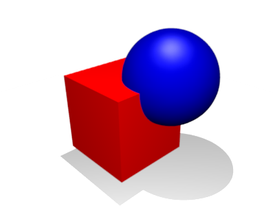
\includegraphics[width=0.3\textwidth]{imgs/Boolean_union}}
  \subfloat[Subtract]{
    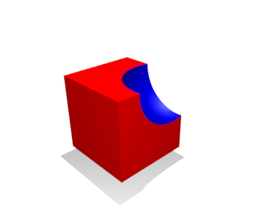
\includegraphics[width=0.3\textwidth]{imgs/Boolean_difference}}
  \subfloat[Intersection]{
    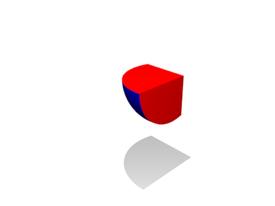
\includegraphics[width=0.3\textwidth]{imgs/Boolean_intersect}}
  \caption{The three different CSG operations in three dimensions. Borrowed from CSGwiki}

  \label{fig:csg}
\end{figure}


\paragraph{Union}
The union Boolean operation merges two interfaces, combining
everything inside the interfaces. This is done by maintaining
everything where the $\phi$-value is below 0. As every pixel contains
the least distance to an interface, the only thing we have to do is to
keep the lowest distance from both input fields and thereby always
having the lowest distance to either of the interfaces.
\begin{equation}
\phi(x,y) = \min(\phi_1(x,y),\phi_2(x,y))
\end{equation}

\paragraph{Intersection}
To get the intersection between two interfaces we remove everything
not contained in either of the interfaces. By keeping the maximum
value from both fields, the pixels inside the first object will get
the distance to the second object. In the intersection the biggest
distance will be the one closest to the edge of the intersection as we
are working with two negative numbers. As we are working with SDFs the
result will also comply with the rules of an SDF.
\begin{equation}
\phi(x,y) = \max(\phi_1(x,y),\phi_2(x,y))
\end{equation}

\paragraph{Subtract}
The subtraction method is also simple. By subtracting the values from
the second field from the first, we maintain the abilities of the SDF
while removing the distances from it in the first. This results in a
new SDF where the interfaces in the second field are removed from the
first.
\begin{equation}
\phi(x,y) = \max(\phi_1(x,y),-\phi_2(x,y))
\end{equation}


%%% Local Variables: 
%%% mode: latex
%%% mode: auto-fill
%%% mode: orgtbl
%%% TeX-PDF-mode: t
%%% TeX-master: "../master.tex"
%%% End: 
